% questions.tex —— 2011 年·江苏卷 · 题目内容片段（无答案）
% 由 tools/generate_projects.py 依来源总账自 2011/2011_数学真题_江苏_试题.md 生成，勿手改（改源 MD 后重跑）

\gkpart{一、填空题}

\begin{question}
\gkti{1}已知集合 $A=\{-1,1,2,4\}$，$B=\{-1,0,2\}$，则 $A\cap B=$ $\underline{\qquad}$。

\end{question}
\begin{question}
\gkti{2}函数 $f(x)=\log_5(2x+1)$ 的单调增区间是 $\underline{\qquad}$。

\end{question}
\begin{question}
\gkti{3}设复数 $z$ 满足 $\mathrm i(z+1)=-3+2\mathrm i$（$\mathrm i$ 是虚数单位），则 $z$ 的实部是 $\underline{\qquad}$。

\Needspace{0.4\textheight}
\end{question}
\begin{question}
\gkti{4}根据如图所示的伪代码，当输入 $a$，$b$ 分别为 $2$，$3$ 时，最后输出的 $m$ 的值是 $\underline{\qquad}$。
\nopagebreak[4]
\begin{center}% 2011 年江苏卷第 4 题：伪代码。
% 来源 PDF：普通高考/2011/2011江苏.pdf，SHA-256 71763ef5d0c2b5800c12515e6b3addb77e585b2460fd11c1013fcec6f050ece9。
% 原页：第 1 页第 1 栏，书页码 675。照原页逐行重排。
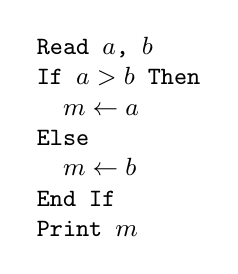
\begin{tikzpicture}[font=\ttfamily\small, semithick]
  \node[anchor=west, align=left] at (0,0) {%
    Read $a$, $b$\\
    If $a>b$ Then\\
    \quad $m\leftarrow a$\\
    Else\\
    \quad $m\leftarrow b$\\
    End If\\
    Print $m$};
\end{tikzpicture}
\end{center}
\nopagebreak[4]
\end{question}
\begin{question}
\gkti{5}从 $1$，$2$，$3$，$4$ 这四个数中一次随机取两个数，则其中一个数是另一个的两倍的概率是 $\underline{\qquad}$。

\end{question}
\begin{question}
\gkti{6}某老师从星期一到星期五收到信件数分别是 $10$，$6$，$8$，$5$，$6$，则该组数据的方差 $s^2=$ $\underline{\qquad}$。

\end{question}
\begin{question}
\gkti{7}已知 $\tan\left(x+\dfrac\pi4\right)=2$，则 $\dfrac{\tan x}{\tan2x}$ 的值为 $\underline{\qquad}$。

\end{question}
\begin{question}
\gkti{8}在平面直角坐标系 $xOy$ 中，过坐标原点的一条直线与函数 $f(x)=\dfrac2x$ 的图象交于 $P$、$Q$ 两点，则线段 $PQ$ 长的最小值是 $\underline{\qquad}$。

\Needspace{0.4\textheight}
\end{question}
\begin{question}
\gkti{9}函数 $f(x)=A\sin(\omega x+\varphi)$（$A$，$\omega$，$\varphi$ 是常数，$A>0$，$\omega>0$）的部分图象如图所示，则 $f(0)=$ $\underline{\qquad}$。
\nopagebreak[4]
\begin{center}% 2011 年江苏卷第 9 题：f(x)=A sin(ωx+φ) 的部分图象。
% 来源 PDF：普通高考/2011/2011江苏.pdf，SHA-256 71763ef5d0c2b5800c12515e6b3addb77e585b2460fd11c1013fcec6f050ece9。
% 原页：第 1 页第 1 栏下部，书页码 675。
% 特征：零点 x=π/3，最小值 -√2 在 x=7π/12（虚线），故 A=√2、ω=2、φ=π/3。
% 横轴以 π 为单位（π 记作 1）。
\begin{tikzpicture}[>=stealth, semithick, font=\small, x=9cm, y=1.5cm]
  \draw[->] (-0.13,0) -- (0.72,0) node[right] {$x$};
  \draw[->] (0,-1.45) -- (0,1.55) node[above] {$y$};
  \node[below left] at (0,0) {$O$};
  \draw[dashed] (7/12,0) -- (7/12,-1.414);
  \draw[dashed] (-0.06,-1.414) -- (7/12,-1.414);
  \node[left] at (-0.005,-1.414) {$-\sqrt2$};
  \node[above] at (1/3,0.03) {$\frac{\pi}{3}$};
  \node[above] at (7/12,0.03) {$\frac{7\pi}{12}$};
  \draw[very thick, domain=-0.10:0.70, samples=240, smooth]
    plot (\x, {1.414*sin(deg(2*pi*\x+pi/3))});
\end{tikzpicture}
\end{center}
\nopagebreak[4]
\end{question}
\begin{question}
\gkti{10}已知 $\boldsymbol e_1$，$\boldsymbol e_2$ 是夹角为 $\dfrac{2\pi}3$ 的两个单位向量，$\boldsymbol a=\boldsymbol e_1-2\boldsymbol e_2$，$\boldsymbol b=k\boldsymbol e_1+\boldsymbol e_2$。若 $\boldsymbol a\cdot\boldsymbol b=0$，则 $k$ 的值为 $\underline{\qquad}$。

\end{question}
\begin{question}
\gkti{11}已知实数 $a\neq0$，函数 $f(x)=\begin{cases}2x+a,&x<1,\\-x-2a,&x\geqslant1.\end{cases}$ 若 $f(1-a)=f(1+a)$，则 $a$ 的值为 $\underline{\qquad}$。

\end{question}
\begin{question}
\gkti{12}在平面直角坐标系 $xOy$ 中，已知点 $P$ 是函数 $f(x)=\mathrm e^x$（$x>0$）的图象上的动点，该图象在 $P$ 处的切线 $l$ 交 $y$ 轴于点 $M$。过点 $P$ 作 $l$ 的垂线交 $y$ 轴于点 $N$。设线段 $MN$ 的中点的纵坐标为 $t$，则 $t$ 的最大值是 $\underline{\qquad}$。

\end{question}
\begin{question}
\gkti{13}设 $1=a_1\leqslant a_2\leqslant\cdots\leqslant a_7$，其中 $a_1$，$a_3$，$a_5$，$a_7$ 成公比为 $q$ 的等比数列，$a_2$，$a_4$，$a_6$ 成公差为 $1$ 的等差数列，则 $q$ 的最小值是 $\underline{\qquad}$。

\end{question}
\begin{question}
\gkti{14}设集合 $A=\left\{(x,y)\ \middle|\ \dfrac m2\leqslant(x-2)^2+y^2\leqslant m^2,\ x,y\in\mathbf R\right\}$，$B=\{(x,y)\mid 2m\leqslant x+y\leqslant2m+1,\ x,y\in\mathbf R\}$。若 $A\cap B\neq\varnothing$，则实数 $m$ 的取值范围是 $\underline{\qquad}$。

\end{question}
\gkpart{二、解答题}

\begin{question}
\gkti{15}在 $\triangle ABC$ 中，角 $A$，$B$，$C$ 所对应的边为 $a$，$b$，$c$。

（1） 若 $\sin\left(A+\dfrac\pi6\right)=2\cos A$，求 $A$ 的值；

（2） 若 $\cos A=\dfrac13$，$b=3c$，求 $\sin C$ 的值。

\Needspace{0.4\textheight}
\end{question}
\begin{question}
\gkti{16}如图，在四棱锥 $P-ABCD$ 中，平面 $PAD\perp$ 平面 $ABCD$，$AB=AD$，$\angle BAD=60^\circ$，$E$，$F$ 分别是 $AP$，$AD$ 的中点。求证：

（1） 直线 $EF\parallel$ 平面 $PCD$；

（2） 平面 $BEF\perp$ 平面 $PAD$。
\nopagebreak[4]
\begin{center}% 2011 年江苏卷第 16 题：四棱锥 P-ABCD。
% 来源 PDF：普通高考/2011/2011江苏.pdf，SHA-256 71763ef5d0c2b5800c12515e6b3addb77e585b2460fd11c1013fcec6f050ece9。
% 原页：第 1 页第 2 栏下部，书页码 675。
% 拓扑：P 在平面 ABCD 上方；E 为 AP 中点、F 为 AD 中点；AD=AB、∠BAD=60°。
\begin{tikzpicture}[>=stealth, semithick, font=\small, scale=0.95]
  \coordinate (A) at (0,0);
  \coordinate (B) at (3.0,0.35);
  \coordinate (D) at (1.35,1.35);
  \coordinate (C) at (4.35,1.70);
  \coordinate (P) at (2.1,4.0);
  \coordinate (E) at ($(A)!0.5!(P)$);
  \coordinate (F) at ($(A)!0.5!(D)$);
  % 底面
  \draw (A)--(B)--(C)--(D)--cycle;
  % 侧棱（可见）
  \draw (P)--(B);
  \draw (P)--(C);
  \draw (P)--(D);
  \draw (P)--(A);
  % 辅助线与中点
  \draw (A)--(C);
  \draw (B)--(D);
  \draw (E)--(F);
  \fill (E) circle (1.4pt) node[above left] {$E$};
  \fill (F) circle (1.4pt) node[left] {$F$};
  \node[above] at (P) {$P$};
  \node[left] at (A) {$A$};
  \node[below] at (B) {$B$};
  \node[right] at (C) {$C$};
  \node[right] at (D) {$D$};
\end{tikzpicture}
\end{center}
\nopagebreak[4]
\Needspace{0.4\textheight}
\end{question}
\begin{question}
\gkti{17}请你设计一个包装盒。如图所示，$ABCD$ 是边长为 $60$ cm 的正方形硬纸片，切去阴影部分所示的四个全等的等腰直角三角形，再沿虚线折起，使得 $A$，$B$，$C$，$D$ 四个点重合于图中的点 $P$，正好形成一个正四棱柱形状的包装盒，$E$，$F$ 在 $AB$ 上，是被切去的等腰直角三角形斜边的两个端点。设 $AE=FB=x$（cm）。

（1） 若广告商要求包装盒侧面积 $S$（cm$^2$）最大，试问 $x$ 应取何值？

（2） 若广告商要求包装盒容积 $V$（cm$^3$）最大，试问 $x$ 应取何值？并求出此时包装盒的高与底面边长的比值。
\nopagebreak[4]
\begin{center}% 2011 年江苏卷第 17 题：正方形硬纸片折叠成正四棱柱包装盒。
% 来源 PDF：普通高考/2011/2011江苏.pdf，SHA-256 71763ef5d0c2b5800c12515e6b3addb77e585b2460fd11c1013fcec6f050ece9。
% 原页：第 1 页第 3 栏上部，书页码 675。示意图，不按比例。
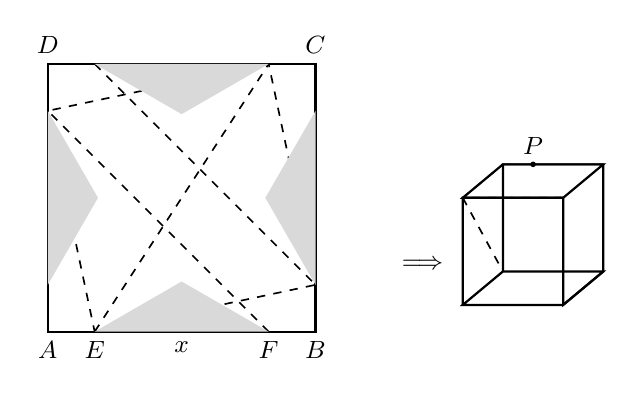
\begin{tikzpicture}[>=stealth, semithick, font=\small, scale=0.85]
  % 左：正方形纸片
  \coordinate (A) at (0,0);
  \coordinate (B) at (4,0);
  \coordinate (C) at (4,4);
  \coordinate (D) at (0,4);
  \coordinate (E) at (0.7,0);
  \coordinate (F) at (3.3,0);
  \coordinate (G) at (4,0.7);
  \coordinate (H) at (3.3,4);
  \coordinate (I) at (0,3.3);
  \coordinate (J) at (0.7,4);
  \draw[thick] (A)--(B)--(C)--(D)--cycle;
  % 折痕
  \draw[dashed] (E)--(G)--(H)--(I)--cycle;
  \draw[dashed] (E)--(H);
  \draw[dashed] (F)--(I);
  \draw[dashed] (J)--(G);
  % 切去的四个等腰直角三角形
  \fill[gray!30] (E)--(F)--(2,0.75)--cycle;
  \fill[gray!30] (J)--(H)--(2,3.25)--cycle;
  \fill[gray!30] (I)--(0.75,2)--(0,0.7)--cycle;
  \fill[gray!30] (G)--(4,3.3)--(3.25,2)--cycle;
  \node[below] at (A) {$A$};
  \node[below] at (B) {$B$};
  \node[above] at (C) {$C$};
  \node[above] at (D) {$D$};
  \node[below] at (E) {$E$};
  \node[below] at (F) {$F$};
  \node[below] at (2,0) {$x$};
  % 右：折成的正四棱柱
  \begin{scope}[xshift=6.2cm, yshift=0.4cm]
    \coordinate (a) at (0,0); \coordinate (b) at (1.5,0);
    \coordinate (c) at (2.1,0.5); \coordinate (d) at (0.6,0.5);
    \coordinate (a1) at (0,1.6); \coordinate (b1) at (1.5,1.6);
    \coordinate (c1) at (2.1,2.1); \coordinate (d1) at (0.6,2.1);
    \draw[thick] (a)--(b)--(c)--(d)--cycle;
    \draw[thick] (a)--(a1)--(b1)--(b)--(c)--(c1)--(d1)--(d);
    \draw[thick] (a1)--(b1)--(c1)--(d1)--cycle;
    \draw[dashed] (d1)--(d);
    \draw[dashed] (a1)--(d);
    \draw[dashed] (b1)--(a1) -- (d1);
    \fill (1.05,2.1) circle (1.2pt) node[above] {$P$};
  \end{scope}
  \node at (5.6,1.0) {$\Longrightarrow$};
\end{tikzpicture}
\end{center}
\nopagebreak[4]
\Needspace{0.4\textheight}
\end{question}
\begin{question}
\gkti{18}如图，在平面直角坐标系 $xOy$ 中，$M$，$N$ 分别是椭圆 $\dfrac{x^2}4+\dfrac{y^2}2=1$ 的顶点，过坐标原点的直线交椭圆于 $P$，$A$ 两点，其中点 $P$ 在第一象限，过 $P$ 作 $x$ 轴的垂线，垂足为 $C$，连接 $AC$，并延长交椭圆于点 $B$，设直线 $PA$ 的斜率为 $k$。

（1） 当直线 $PA$ 平分线段 $MN$ 时，求 $k$ 的值；

（2） 当 $k=2$ 时，求点 $P$ 到直线 $AB$ 的距离 $d$；

（3） 对任意 $k>0$，求证：$PA\perp PB$。
\nopagebreak[4]
\begin{center}% 2011 年江苏卷第 18 题：椭圆 x^2/4 + y^2/2 = 1 与点 M,N,P,A,B,C。
% 来源 PDF：普通高考/2011/2011江苏.pdf，SHA-256 71763ef5d0c2b5800c12515e6b3addb77e585b2460fd11c1013fcec6f050ece9。
% 原页：第 1 页第 3 栏下部，书页码 675。按题设取 k=1 示意。
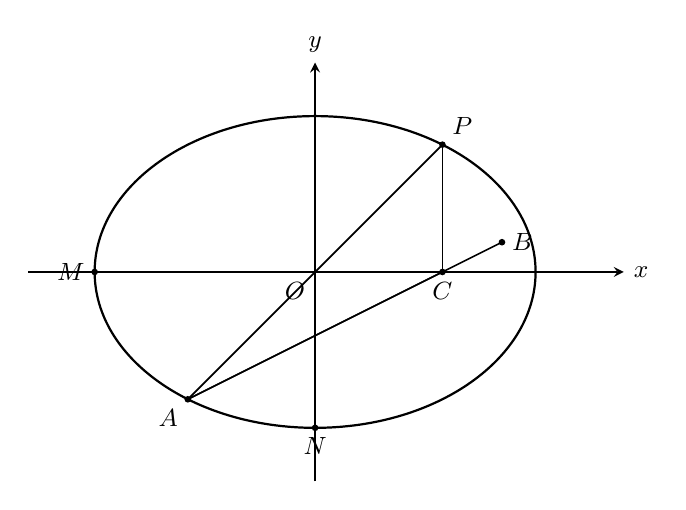
\begin{tikzpicture}[>=stealth, semithick, font=\small, x=1.4cm, y=1.4cm]
  \draw[->] (-2.6,0) -- (2.8,0) node[right] {$x$};
  \draw[->] (0,-1.9) -- (0,1.9) node[above] {$y$};
  \node[below left] at (0,0) {$O$};
  \draw[thick] (0,0) ellipse ({2} and {1.414});
  \coordinate (O) at (0,0);
  \coordinate (M) at (-2,0);
  \coordinate (N) at (0,-1.414);
  \coordinate (P) at (1.155,1.155);
  \coordinate (C) at (1.155,0);
  \coordinate (A) at (-1.155,-1.155);
  \coordinate (B) at (1.695,0.270);
  \draw (P)--(O)--(A);
  \draw (P)--(C);
  \draw (A)--(B);
  \draw (A)--(C);
  \fill (M) circle (1.2pt) node[left] {$M$};
  \fill (N) circle (1.2pt) node[below] {$N$};
  \fill (P) circle (1.2pt) node[above right] {$P$};
  \fill (A) circle (1.2pt) node[below left] {$A$};
  \fill (B) circle (1.2pt) node[right] {$B$};
  \fill (C) circle (1.2pt) node[below] {$C$};
\end{tikzpicture}
\end{center}
\nopagebreak[4]
\end{question}
\begin{question}
\gkti{19}已知 $a$，$b$ 是实数，函数 $f(x)=x^3+ax$，$g(x)=x^2+bx$，$f'(x)$ 和 $g'(x)$ 分别是 $f(x)$，$g(x)$ 的导函数，若 $f'(x)g'(x)\geqslant0$ 在区间 $I$ 上恒成立，则称 $f(x)$ 和 $g(x)$ 在区间 $I$ 上单调性一致。

（1） 设 $a>0$，若函数 $f(x)$ 和 $g(x)$ 在区间 $[-1,+\infty)$ 上单调性一致，求实数 $b$ 的取值范围；

（2） 设 $a<0$ 且 $a\neq b$，若 $f(x)$ 和 $g(x)$ 在以 $a$，$b$ 为端点的开区间上单调性一致，求 $|a-b|$ 的最大值。

\end{question}
\begin{question}
\gkti{20}设 $M$ 为部分正整数组成的集合，数列 $\{a_n\}$ 的首项 $a_1=1$，前 $n$ 项和为 $S_n$，已知对任意整数 $k\in M$，当整数 $n>k$ 时，$S_{n+k}+S_{n-k}=2(S_n+S_k)$ 都成立。

（1） 设 $M=\{1\}$，$a_2=2$，求 $a_5$ 的值；

（2） 设 $M=\{3,4\}$，求数列 $\{a_n\}$ 的通项公式。

\end{question}
\gkpart{三、附加题}

\Needspace{0.4\textheight}
\begin{question}
\gkti{21}四选二。

【A】如图，圆 $O_1$ 与圆 $O_2$ 内切于点 $A$，其半径分别为 $r_1$ 与 $r_2$（$r_1>r_2$），圆 $O_1$ 的弦 $AB$ 交圆 $O_2$ 于点 $C$（$O_1$ 不在 $AB$ 上），求证：$AB:AC$ 为定值。
\nopagebreak[4]
\begin{center}% 2011 年江苏卷附加题 21A：两圆内切于点 A，圆 O1 的弦 AB 交圆 O2 于 C。
% 来源 PDF：普通高考/2011/2011江苏.pdf，SHA-256 71763ef5d0c2b5800c12515e6b3addb77e585b2460fd11c1013fcec6f050ece9。
% 原页：第 2 页第 2 栏，书页码 676。r1:r2 示意取 2.2:1.3。
\begin{tikzpicture}[>=stealth, semithick, font=\small, scale=0.9]
  \coordinate (O1) at (0,0);
  \coordinate (O2) at (0.9,0);
  \coordinate (A) at (2.2,0);
  \coordinate (B) at (-1.1,1.905);
  \draw[thick] (O1) circle (2.2);
  \draw[thick] (O2) circle (1.3);
  \draw (A)--(B);
  \fill (O1) circle (1.2pt) node[below] {$O_1$};
  \fill (O2) circle (1.2pt) node[below] {$O_2$};
  \fill (A) circle (1.2pt) node[right] {$A$};
  \fill (B) circle (1.2pt) node[above left] {$B$};
  \coordinate (C) at ($(A)!0.56!(B)$);
  \fill (C) circle (1.2pt) node[below right] {$C$};
\end{tikzpicture}
\end{center}
\nopagebreak[4]
【B】已知矩阵 $A=\begin{bmatrix}1&1\\2&1\end{bmatrix}$，向量 $\boldsymbol\beta=\begin{bmatrix}1\\2\end{bmatrix}$，求向量 $\boldsymbol\alpha$，使得 $A^2\boldsymbol\alpha=\boldsymbol\beta$。

【C】在平面直角坐标系 $xOy$ 中，求过椭圆 $\begin{cases}x=5\cos\varphi,\\y=3\sin\varphi\end{cases}$（$\varphi$ 为参数）的右焦点，且与直线 $\begin{cases}x=4-2t,\\y=3-t\end{cases}$（$t$ 为参数）平行的直线的普通方程。

【D】解不等式：$x+|2x-1|<3$。

\Needspace{0.4\textheight}
\end{question}
\begin{question}
\gkti{22}如图，在正四棱柱 $ABCD-A_1B_1C_1D_1$ 中，$AA_1=2$，$AB=1$，点 $N$ 是 $BC$ 的中点，点 $M$ 在 $CC_1$ 上。设二面角 $A_1-DN-M$ 的大小为 $\theta$。

（1） 当 $\theta=90^\circ$ 时，求 $AM$ 的长；

（2） 当 $\cos\theta=\dfrac{\sqrt6}6$ 时，求 $CM$ 的长。
\nopagebreak[4]
\begin{center}% 2011 年江苏卷附加题 22：正四棱柱 ABCD-A1B1C1D1，N 为 BC 中点，M 在 CC1 上。
% 来源 PDF：普通高考/2011/2011江苏.pdf，SHA-256 71763ef5d0c2b5800c12515e6b3addb77e585b2460fd11c1013fcec6f050ece9。
% 原页：第 2 页第 3 栏，书页码 676。AA1=2，AB=1，示意不按比例。
\begin{tikzpicture}[>=stealth, semithick, font=\small, scale=0.95]
  \coordinate (A) at (0,0);
  \coordinate (B) at (2.0,0.15);
  \coordinate (C) at (2.8,1.05);
  \coordinate (D) at (0.8,0.9);
  \coordinate (A1) at (0.35,2.5);
  \coordinate (B1) at (2.35,2.65);
  \coordinate (C1) at (3.15,3.55);
  \coordinate (D1) at (1.15,3.4);
  \coordinate (N) at ($(B)!0.5!(C)$);
  \coordinate (M) at ($(C)!0.45!(C1)$);
  \draw[thick] (A)--(B)--(C)--(D)--cycle;
  \draw[thick] (A)--(A1) (B)--(B1) (C)--(C1) (D)--(D1);
  \draw[thick] (A1)--(B1)--(C1)--(D1)--cycle;
  \draw[dashed] (A1)--(D);
  \draw[dashed] (D)--(D1);
  \draw[dashed] (A1)--(D1);
  \draw (A1)--(N);
  \draw (D)--(N);
  \draw (D)--(M);
  \draw (N)--(M);
  \fill (N) circle (1.2pt) node[below right] {$N$};
  \fill (M) circle (1.2pt) node[right] {$M$};
  \node[below left] at (A) {$A$};
  \node[below] at (B) {$B$};
  \node[right] at (C) {$C$};
  \node[left] at (D) {$D$};
  \node[left] at (A1) {$A_1$};
  \node[above] at (B1) {$B_1$};
  \node[right] at (C1) {$C_1$};
  \node[above] at (D1) {$D_1$};
\end{tikzpicture}
\end{center}
\nopagebreak[4]
\end{question}
\begin{question}
\gkti{23}设整数 $n\geqslant4$，$P(a,b)$ 是平面直角坐标系 $xOy$ 中的点，其中 $a$，$b\in\{1,2,3,\cdots,n\}$，$a>b$。

（1） 记 $A_n$ 为满足 $a-b=3$ 的点 $P$ 的个数，求 $A_n$；

（2） 记 $B_n$ 为满足 $\dfrac13(a-b)$ 是整数的点 $P$ 的个数，求 $B_n$。

\end{question}